% MySubmissionMainAtJournMathMusic.tex
% v1.1 prepared by Thomas Fiore
% Thomas Fiore retains the copyright for content this template.

% This file is the author template for the author's main submission file at the Journal of Mathematics and Music
% Online Supplement (if needed) has a different template, use the other template for Online Supplements in this folder.

%%%%%%%%%%%%%%%%%% NOTE TO AUTHORS%%%%%%%%%%%%%
% Please use this template to prepare your submission PDF. Save all files from the Author Package in one folder so they work in sync, this folder is called your ``working directory.''
% Do not include your name in the file-name because the file-name displays in the compiled PDF at the top at the top of every page. Your name should not be included there in order to guarantee double-blind reviewing.
% After reading the pre-compiled pdf file, rename this LaTeX file, follow the directions in these comments, and fill in the blanks according to the comment lines in this file.
% This file is the quick-start LaTeX template for you. More detailed instructions are in the tMAMguide.pdf file if needed.
% IMPORTANT: After you finish your draft, but before submission, please read again all the Punctation Tips and Coding Tips in the template PDF and verify that your manuscript follows them. This will speed up the reviewing, editing, and production of your manuscript (if accepted).
% Use PDFLaTex and BibTex to compile. PDFLaTeX is necessary to create the hyperlinks.
% If there is a conflict in formal aspects between the tMAMguide.pdf and this template, follow the format in this template,
% not tMAM.guide.pdf.
%%%%%%%%%%%%%%%%%%%%%%%%%%%%%%%%%%%%%%%%%%%%%%%%%

\documentclass{tMAM2e}% Use this class file. Do not change this line. This class file must be in your working directory.


\usepackage{epstopdf}% To incorporate .eps illustrations using PDFLaTeX, etc.
\usepackage[bookmarksnumbered,colorlinks,bookmarks,citecolor=blue,linkcolor=blue,urlcolor=blue,breaklinks,linktocpage]{hyperref}% To create hyperlinks using PDFLaTeX, etc.
\usepackage[all]{hypcap}% This turns on the hyperlinks for \label{} and \ref{}, and others.
\usepackage{subfigure}% Support for small, `sub' figures and tables

\theoremstyle{plain}
\newtheorem{theorem}{Theorem}[section]
\newtheorem{corollary}[theorem]{Corollary}
\newtheorem{lemma}[theorem]{Lemma}
\newtheorem{proposition}[theorem]{Proposition}

\theoremstyle{definition}
\newtheorem{definition}[theorem]{Definition}

\theoremstyle{remark}
\newtheorem{remark}[theorem]{Remark}
\newtheorem{example}[theorem]{Example}

\usepackage{color}
\newcommand{\anonymized}{{\color{red}\emph{anonymized}}}
\newcommand{\suppl}[1]{Online Supplement §#1}

\begin{document}

% The following two lines are for production department only. Do not change.
%\jvol{00} \jnum{00} \jyear{2015}
%\doi{insert doi link}

% If this is an Editorial by guest editors, uncomment the next line. If this is a research article, do not change anything,
% since research article is the default and we do not mark articles as ``research articles'' anymore
%\articletype{EDITORIAL}

% Replace the title below by your title. Only the first letter and proper names are capitalized.
\title{Rhythmic segment analysis:\\
Conceptualizing, visualizing, and measuring rhythmic data}

\author{
% \name{Bas Cornelissen\textsuperscript{a}$^{\ast}$\thanks{$^\ast$Corresponding author. Email: mail@bascornelissen.nl}}
%
% @EDITOR: I hope you forgive me for adding a linebreak after the institute; improves the balance
%
% \affil{\textsuperscript{a}Institute for Logic, Language and Computation,\\
% University of Amsterdam, Amsterdam, The~Netherlands}
%leave blank for production:
\received{}
}

\maketitle

% Abstract
\begin{abstract}
This paper addresses how to conceptualize, visualize, and measure regularities in rhythmic data.
I propose to think about rhythmic data in terms of interval segments: fixed-length groups of consecutive intervals, which can be decomposed into a duration and a pattern, the latter being a point in a rhythm simplex (e.g. $1 : 1 : 2$). 
This simple conceptual framework unifies three rhythmic visualization methods and suggests a fourth: the pattern-duration plot. 
When paired with a cluster transition network, it intuitively reveals regularities in both synthetic and real-world rhythmic data. 
Moreover, the framework generalizes two common measures of rhythmic structure: rhythm ratios and the normalized pairwise variability index (nPVI). 
In particular, nPVI can be reconstructed as the average distance from isochrony, and I propose a more general measure of anisochrony to replace it. 
Finally, the novel concept of quantal data proves to be fruitful. 
Referring to intervals that cluster around integer multiples of a smallest duration, it may shed light on wider debates regarding small integer ratio rhythms. 
The presentation in the paper is relatively informal, a more formal presentation is given in the Online Supplement.
\end{abstract}

% Keywords
\begin{keywords}
rhythmic segment analysis; rhythm ratio; isochrony; anisochrony; nPVI; quantal data
\end{keywords}

% AMS MSC and MCM CCS
\begin{classcode}\textit{2020 Mathematics Subject Classification}: 00A65 \\
\textit{2012 Computing Classification Scheme}: applied computing
\end{classcode}


%%%%%%%%%%%%%%%%%%%%%%%%%%%%%%%%%%%%%%%%%%%%%%%%%%%%%%%%%%%%%%%%%%%%%%%%%%%%%%%%%%%%%
%%%%%%%%%%%%%%%%%%%%%%%%%%%%%%%%%%%%%%%%%%%%%%%%%%%%%%%%%%%%%%%%%%%%%%%%%%%%%%%%%%%%%

\noindent%
Without rhythm, no music—let alone music cognition. 
Yet it appears that the field lacks a compelling conceptual framework for reasoning about rhythmic data. 
Suppose we are presented with some rhythmic data: intervals between drum-stroke onsets perhaps. 
How might we determine whether regularities are present? How might we characterize them? 
%
Even the “most empirically suitable approach to quantify rhythmic structure” \citep{Ravignani2017MusicPercept}, the normalized pairwise variability index (nPVI), has received substantial methodological criticism \citep{Condit-Schultz2019MusicPercept} and is rather limited in what structure it can describe: only isochrony, as we will see. 
A series of recent studies, some at the interface with bioacoustics, has been addressing this gap by proposing novel visualizations and measures of rhythmic structure \citep{Burchardt2025OSF, Jadoul2025Vibration, Ravignani2017MusicPercept, Roeske2020CurrBiol}. 


The starting point for this paper is a simple observation. 
All of these studies analyze the same objects: interval pairs. 
That means that multiple visualization methods (phase, ratio, and raster plots) and rhythmic measures (rhythm ratios and the nPVI) can be unified in a single theoretical framework that generalizes the notion of an interval pair. 
The goal of this paper is to develop that framework, and nothing more. 
Since the focus is narrow, I will not review the literature at large but refer to other sources for broader surveys \citep{Burchardt2025OSF,Jadoul2025Vibration,VanHandel2022}. 

This paper, in short, addresses how to (1) conceptualize, (2) visualize, and (3) measure regularities in rhythmic data. 
The approach I put forward, \emph{rhythmic segment analysis}, is summarized in Figure~\ref{fig:rsa}. 
It conceptualizes rhythmic data in terms of its \emph{segments}: fixed-length groups of consecutive intervals, like interval pairs or triplets such as $(0.2, 0.2, 0.4)$. 
Segments will be decomposed into a \emph{duration} and a \emph{pattern}, the latter being the ratios between the intervals in a segment (e.g. 
$1 : 1 : 2$). 
Multiple existing plotting methods turn out to visualize segments or patterns, and I propose a more effective method: the pattern-duration plot. 
When overlaid with a network summarizing segment transitions, it can intuitively reveal rhythmic regularities in a dataset. 
Finally, this framework naturally incorporates two measures of rhythmic regularity. 
First, rhythm ratios correspond directly to length-2 patterns. 
Second, the nPVI naturally emerges as an average distance from isochrony, and leads to a more general (and normalized) measure of anisochrony that can replace the nPVI.

The strength of the proposed framework is its simplicity and generality. 
Rhythmic segment analysis naturally ties together existing work, can help clarify our reasoning about rhythmic data, and is straightforward to implement: (1) split intervals into fixed-length segments, (2) sum them, and then (3) normalize the segments to get durations and patterns. 
A small Python package, \anonymized{},
%\emph{rhythmic-segments},
which I release alongside this paper simplifies things even further, especially when it comes to handling metadata. 
Installation instructions and extensive documentation are available online, as are all the data and code discussed in this paper.\footnote{%
  The package \anonymized{}
  % \emph{rhythmic-segments} 
  can be installed using pip, and the documentation can be found at 
  \anonymized{}.github.io/\anonymized{}.
  % bacor.github.io/rhythmic-segments.
  All data and code used in this paper, along with the supplementary materials, have been deposited at doi.org/10.5281/zenodo.\anonymized{}.
  %17753529. 
}

\begin{figure}
  \begin{center}
  \resizebox*{12cm}{!}{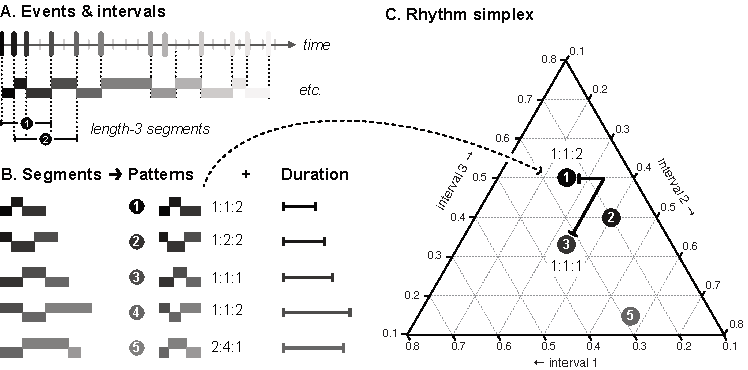
\includegraphics{../../figures/rsa-summary.pdf}}\\
  \caption{%
    \textbf{Rhythmic segment analysis} studies fixed-length segments of interval data, illustrated in panel \textbf{(A)} with segments of 3 intervals. 
    Intervals alternate up or down for readability. 
    \textbf{(B)} Segments can be decomposed into a pattern (e.g. $1 : 1 : 2$) and a duration, with patterns falling in a space known as the rhythm simplex (Section~\ref{sec:conceptualization}). 
    \textbf{(C)}  This decomposition allows one to visualize rhythmic data effectively (Section~\ref{sec:visualization}), and to quantify its characteristics (e.g. 
    its isochronicity) using suitable distance metrics on the simplex (Section~\ref{sec:measurement}).%
  }
  \label{fig:rsa}
  \end{center}
\end{figure}


%==========================
\section{Conceptualization}%
\label{sec:conceptualization}
%==========================


I would like to start by simply laying out the basic ingredients of a rhythmic segment analysis. 
To address a wide audience, I will introduce the key concepts with examples and geometric intuitions wherever possible. 
A more formal exposition is provided in the Online Supplement.

\subsection{Segments, patterns, and durations}
The starting point is ‘rhythmic data’, which here refers to a sequence of events: points in time without duration. 
We often ignore the events themselves and consider only the time \emph{intervals} between them. 
This is consistent with the most typical use case, where events are note onsets and the data consists of inter-onset intervals. 
Moreover, the motivating use case is one where the events are measured in continuous time—onsets from a recording rather than a score.

The idea is to analyze rhythmic data in terms of its segments: groups of consecutive intervals obtained by sliding a fixed-length window over the intervals (interval $n$-grams, in short). 
For example, the length-3 segments of the intervals $(.1, .1, .2, .2, .2, .4, .3, \dots)$ would be $(.1, .1, .2)$, $(.1, .2, .2)$, $(.2, .2, .2)$, $(.2, .2, .4)$, and so on. 
Segments like $(.1, .1, .2)$ and $(.2, .2, .4)$ have different \emph{duration}—0.4s and 0.8s respectively—but both represent the same \emph{pattern}: short, short, twice as long. 
This pattern can be described formally by either the \emph{ratios} between the intervals, $1 : 1 : 2$, or by their \emph{relative durations} $(.25, .25, .5)$. 
Both descriptions are equivalent and can be used interchangeably. 

Simple as it may be, this is an important point: segments can be decomposed into durations and patterns. 
Doing so effectively isolates tempo, in the form of a duration, from the segments’ rhythmic ‘content’. 
The remaining pattern describes that content in terms of the relations between intervals irrespective of their absolute durations (or tempo)—similar perhaps to how relative pitch might describe relations between notes irrespective of their absolute frequencies. 


\begin{figure}
  \begin{center}
  \resizebox*{6cm}{!}{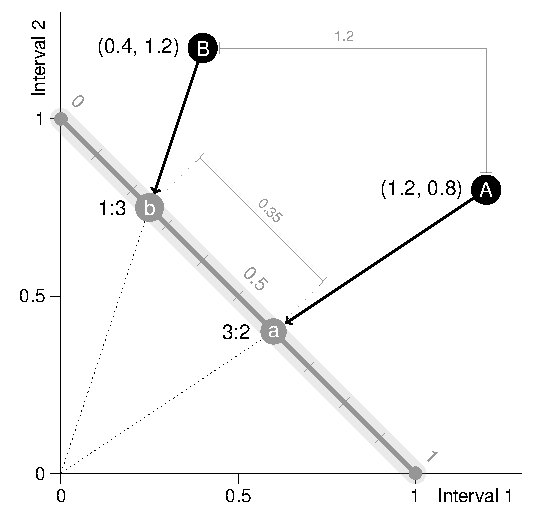
\includegraphics{../rsa-2d-simplex.pdf}}\\
  \caption{%
    \textbf{The rhythm line.}
    Two length-2 segments, $A$ and $B$, are shown by plotting the first against the second interval. 
    The rhythm simplex is the thick gray line and represents all possible length-2 patterns. 
    Values along the simplex indicate rhythm ratios $r$, isochrony corresponds to $r = 0.5$. 
    Normalizing segments $A$ and $B$ projects them onto the simplex, producing patterns $a$ and $b$ with ratios $1 : 3$ (at $r = 0.25$ in the simplex) and $3 : 2$ (at $r = 0.6$) respectively. 
    All segments on the same line through the origin have the same pattern. 
    The segment distance between $A$ and $B$ is the length of the shortest path over grid lines (solid gray line, $1.2$), while the pattern distance between a and b is the shortest path within the simplex ($0.35$).%
  }
  \label{fig:rhythm-line}
  \end{center}
\end{figure}



\subsection{The rhythm simplex}
%——————————————————————————————
Patterns are effectively normalized segments. 
To continue the example, entries of the pattern $(0.25, 0.25, 0.5)$ sum to one, and the last entry is therefore fully determined by the others: it equals one minus their sum. 
A pattern of length three consequently has only two ‘degrees of freedom’. 
By the same logic, patterns of length n must form an $(n - 1)$-dimensional space. 
The space of patterns was first studied by \citet{Desain2003Perception} and will be referred to here as the \emph{rhythm simplex} following \citet{Jacoby2017CurrBiol}. 
Each point in that space represents a rhythmic pattern.

Figure~\ref{fig:rhythm-line} illustrates what one may call the rhythm line: the simplex of length-2 patterns (i.e. for two intervals between three events). 
A value of $0.2$ along that line corresponds to the pattern $(0.2, 1 - 0.2) = (0.2, 0.8)$ or the ratio $1 : 4$. 
The value describes the relative duration of the first interval and is also known as the rhythm ratio $r$ or $r_k$ introduced by \citet{Roeske2020CurrBiol}. 
Of particular importance is the value $r = 0.5$. 
It indicates the isochronous pattern $(0.5, 0.5)$ or $1 : 1$, in which all intervals have the same duration. 
Figure~\ref{fig:rhythm-line} shows that normalizing a segment projects it onto the simplex. 
Consequently, all segments on a single line through the origin represent the same pattern. 
The farther they lie from the origin, the slower their tempo. 
(Indeed, the pattern and duration behave exactly like polar coordinates; see the Online Supplement.)

All this generalizes to higher dimensions, as Figure~\ref{fig:rhythm-triangle} shows for the rhythm triangle: the simplex for length-3 patterns (of three intervals between four onsets). 
This triangle was first introduced as the \emph{chronotopic map} by \citet{Desain2003Perception} in a study of categorical rhythm perception. 
More recently, it featured prominently in studies of perceptual priors of listeners from different cultures \citep{Jacoby2017CurrBiol,Jacoby2024NatHumBehav}.
In the center of the simplex, we find the isochronous pattern $(\tfrac{1}{3}, \tfrac{1}{3}, \tfrac{1}{3})$ or $1 : 1 : 1$. 
As one approaches the corners, the patterns become increasingly non-isochronous, approaching the impossible pattern where one interval fills the entire segment and the two others are vanishingly small (e.g. $1 : 0 : 0$).


\begin{figure}
  \begin{center}
  \resizebox*{6cm}{!}{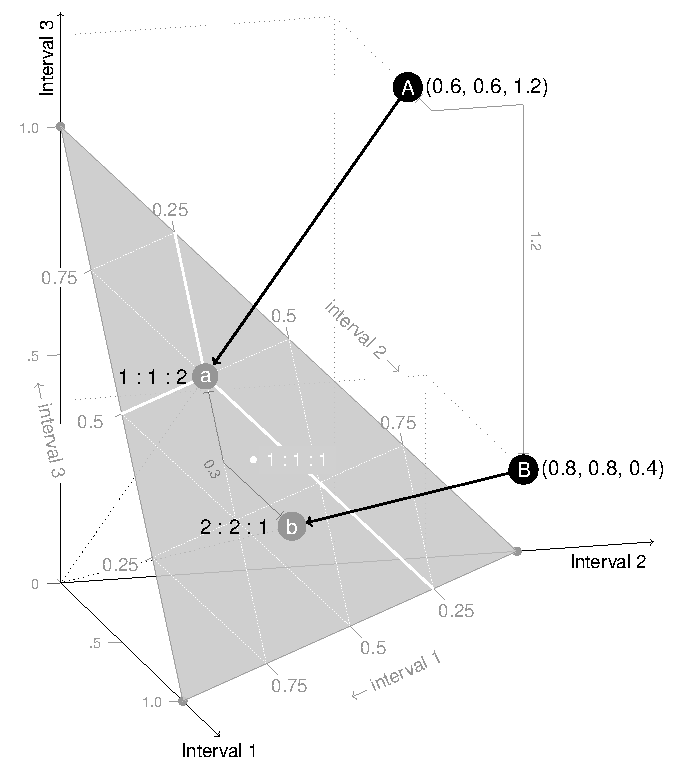
\includegraphics{../rsa-3d-simplex.pdf}}\\
  \caption{%
    \textbf{The rhythm triangle} is the simplex of length-3 patterns. 
    Similar to Figure~\ref{fig:rhythm-line}, normalizing two segments (now interval triplets) projects them onto the triangular simplex (gray). 
    The white ‘crosshair’ shows how to read coordinates of pattern $a$, $(0.25, 0.25, 0.5)$, inside the triangle. 
    The isochronous pattern $1 : 1 : 1$ is shown in the center. 
    Like the segment distance (gray line, $1.2$), the pattern distance is the length of the shortest path ($0.3$), but following the grid lines of the simplex.% 
  }
  \label{fig:rhythm-triangle}
  \end{center}
\end{figure}


\subsection{Measuring distances}
%———————————————————————————————
For length-4 patterns, the rhythm simplex is a tetrahedron. 
Beyond that, the space becomes increasingly hard to visualize. 
But longer segments and patterns can also be studied using suitable distance metrics. 
Instead of Euclidean distance, the \emph{segment distance} I propose is the sum of the absolute differences between two segments. 
This measures the total adjustment needed to turn one segment into the other. 
For example, the segment distance between $(1, 2, 3)$ and $(4, 5, 6)$ is $|1 - 4| + |2 - 5| + |3 - 6| = 9$—seconds, perhaps. 
Geometrically, the segment distance is the length of the shortest path between two segments, provided the path follows the grid lines (see Figures~\ref{fig:rhythm-line} and \ref{fig:rhythm-triangle}). 
For that reason, it is also known as the \emph{taxicab distance}: it measures the path a taxi would take in a grid-like city. 

One could compare patterns in the same way. 
However, because patterns are normalized, the segment distance effectively counts all differences twice: the patterns $(0.25, 0.75)$ and $(0.75, 0.25)$ would appear to be $0.5 + 0.5 = 1$ apart, but when increasing the first interval by $0.5$, normalization already implies an equal change to the second. 
Therefore using half of the segment distance as the pattern distance is more appropriate—formally this is known as the \emph{total variation distance}. 
The pattern distance also measures the shortest path between two patterns, but now it must follow the grid of the simplex (Figures~\ref{fig:rhythm-line} and \ref{fig:rhythm-triangle}). 
Moreover, it is itself normalized, so that the distance between any two corners of the simplex is 1.


%======================
\section{Visualization}%
\label{sec:visualization}
%======================


Rhythmic segments and patterns can have arbitrary length, but only pairs and triplets can be effectively visualized in two dimensions without resorting to dimensionality reduction techniques. 
Such techniques can be very useful, but I first want to address direct visualization. 
It turns out that three existing plotting methods can be understood as segment or pattern plots. 
Moreover, the framework sketched above suggests a fourth plot, the pattern-duration plot, that combines strengths of the other three. 


\subsection{Quantality}
%——————————————————————

We compare these visualization methods using synthetic data whose properties we can fully control and understand. 
One synthetic dataset is of such special interest as a baseline for musical rhythm that I want to propose a term and definition for it. 
I will call rhythmic data \emph{quantal} when the interval distribution consists of clusters close to integer multiples of a smallest temporal unit, the \emph{quantum}. 
In such data, time is approximately discrete: events roughly coincide with a pulse or grid corresponding to the quantum. 
As a result, in a quantal dataset all intervals are approximately related by integer ratios. 
(Stronger still, quantality is equivalent to the presence of integer ratio segment clusters; see \suppl{1.4}.)

There are ample candidates for the quantum (beat, subdivision, tatum, and so on), but I choose a neutral, domain-general term to avoid theoretical baggage and because, depending on the data, the quantum could be any of those. 
Also note that I avoid the term quantization (discretizing continuous intervals to a grid) because the notions are not equivalent: quantal data need not be quantized, but quantized data are always quantal. 


\subsection{Synthetic rhythmic data}
%———————————————————————————————————
I will use three synthetic datasets. 
First, intervals sampled uniformly between $0.2$ and $2$s. 
Second, random small-integer multiples (sampled from a geometric distribution) of a quantum of $0.2$s with some Gaussian noise (e.g. $0.21, 0.42, 0.19, 0.61, \dots$). 
Third, noisy repetitions of a fixed rhythm using a quantum of $0.5$s. 
The Online Supplement describes these and additional examples in more detail. 
All three datasets are continuous, but only the last two are quantal: those contain, by approximation, a limited number of possible intervals and therefore exhibit clear rhythmic categories.


\begin{figure}
  \begin{center}
  \resizebox*{12cm}{!}{%
    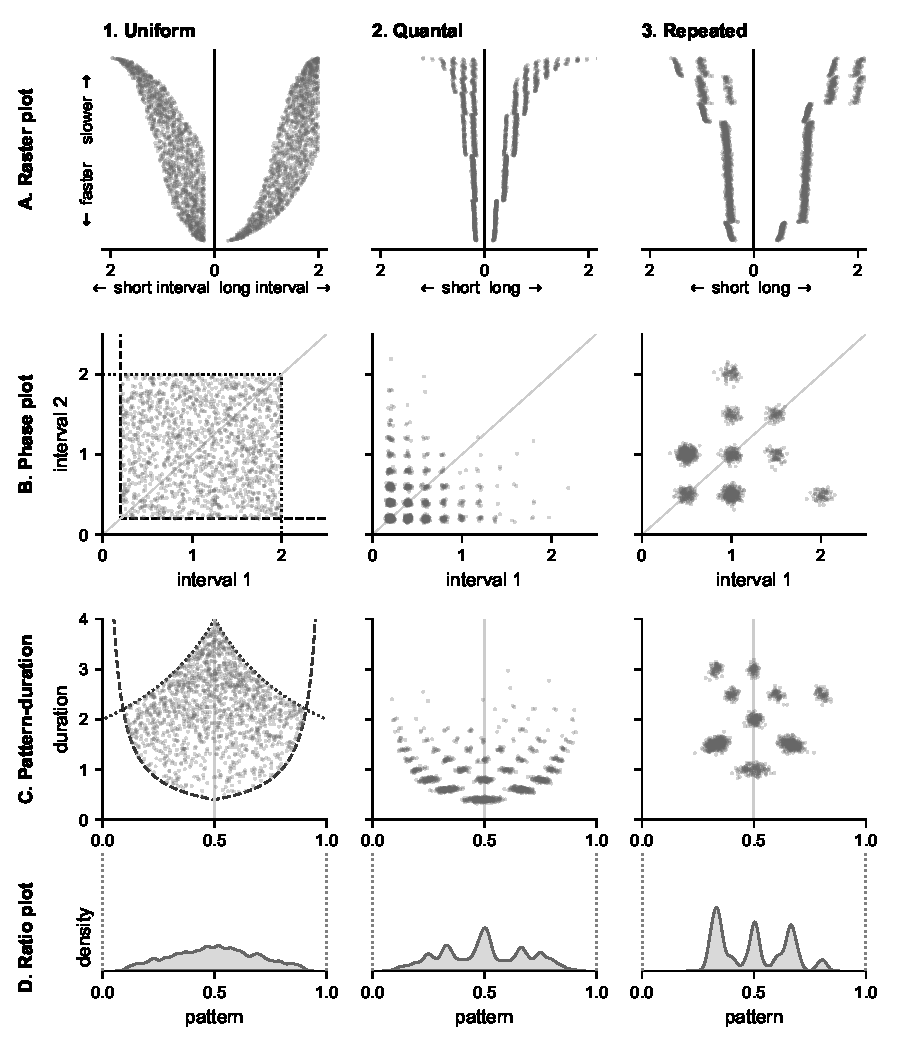
\includegraphics{../../figures/synthetic-data-combined.pdf}%
  }\\
  \caption{%
    \textbf{Length-2 segments of synthetic data visualized in four ways.} 
    Columns show three types of synthetic rhythmic data discussed in the main text: \textbf{(1)} uniform intervals, \textbf{(2)} quantal intervals (noisy integer multiples of a pulse), and \textbf{(3)} a noisy, repeated rhythm. 
    Raster plots \textbf{(A)} sort segments vertically by their duration; the shorter interval of each segment is plotted to the left, the longer one to the right. 
    Phase plots \textbf{(B)} plot the first against the second interval. 
    Pattern-duration plots \textbf{(C)} transform phase plots, mapping every diagonal line to a vertical line: the pattern is represented horizontally by the rhythm ratio and vertically by the segment. 
    Gray lines show isochrony (diagonal in B, vertical line at $0.5$ in C), dashed and dotted lines show the minimum and maximum duration boundaries in both B and C. 
    A ratio plot \textbf{(D)} is a marginal density plot of a pattern-duration plot.%
  }
  \label{fig:plots}
  \end{center}
\end{figure}


\subsection{Phase, raster, and ratio plots}
%——————————————————————————————————————————
First, \emph{raster plots} \citep[][see Figure~\ref{fig:plots}A]{Roeske2020CurrBiol} are the most intriguing and elusive of these plots. 
Segments are sorted vertically by their duration, so that the slowest segments are on top and the fastest at the bottom. 
Each segment is then plotted using two points: the shorter interval on the left and the longer interval on the right. 
Raster plots produce beautiful flower-like figures with richly patterned petals (Figure~\ref{fig:plots}A-3). 
The flower shape, however, is an artefact. 
It appears even for uniform data (see Figure~\ref{fig:plots}A-1), demonstrating that raster plots make inefficient use of visual space. 
Moreover, interpreting the patterning inside the petals is difficult, hampered by the fact that the vertical axis has no scale and that sorting blows up frequent segments.

Second, \emph{phase plots} \citep[][see Figure~\ref{fig:plots}B]{Ravignani2017MusicPercept,Ravignani2016NatHumBehav} present a more interpretable alternative. 
Like Figure~\ref{fig:rhythm-line}, the first interval of each segment is shown along the horizontal axis, the second interval along the vertical axis. 
When the data contain recurrent regularities, connecting successive segments with lines will produce geometric figures (see \suppl{2}).
I have omitted those lines in Figure~\ref{fig:plots}B, as they would also obscure the segment clusters. 
All segments on a line through the origin have the same pattern, with the diagonal representing isochrony. 
The further from the origin, the longer the duration. 
Phase plots also illustrate that quantal data are grid-like in the sense that its segments will cluster around grid points of a quantum-spaced grid (Figure~\ref{fig:plots}B-2).

Third, \emph{ratio plots} \citep[][see Figure~\ref{fig:plots}D]{Roeske2020CurrBiol} show the distribution of rhythm ratios (i.e. length-2 patterns) over the rhythm line using a kernel density estimate. 
Ratio plots have been used in studies of categoricity in rhythmic data \citep[e.g.]{DeGregorio2021CurrBiol}, but they can misrepresent the clustering structure of the data. 
For example, the ratio plot suggests that the repeated dataset has around three rhythmic categories (Figure~\ref{fig:plots}D-3), while the phase plot shows that there are many more segment clusters (Figure~\ref{fig:plots}B-3). 
The ratio plot collapses multiple segment clusters even when these clusters have distinct patterns, such as $1 : 2$ and $2 : 3$ (\suppl{1.4} contains a more dramatic example).
All this is immediately obvious from the pattern-duration plot shown in Figure~\ref{fig:cluster-transition-network}, and which I will introduce now.


\subsection{Pattern-duration plots}
%——————————————————————————————————
Pattern-duration plots show the duration of each segment vertically, against its pattern (the rhythm ratio) horizontally. 
This means that the horizontal marginal density plot of a pattern-duration plot is, in fact, a ratio plot (see the top of Figure~\ref{fig:cluster-transition-network}).
Pattern-duration plots are very closely related to the tempo-ratio plots in \citet{Roeske2020CurrBiol}—which show only half the simplex, as discussed below—as well as phase plots. 
In fact, decomposing a segment into its pattern and duration is a coordinate transform that maps a phase plot to a pattern-duration plot (see \suppl{1.2}).
For example, it maps the isochronous diagonal to the vertical line r = 0.5 (Figures~\ref{fig:plots}B and \ref{fig:plots}C). 
Intuitively, the transform rotates a phase plot by 45 degrees and blows up the area close to the origin. 
The benefit of this transformation is threefold: (1) it makes efficient use of visual space by blowing up a typically dense region around rapid, approximate isochrony; (2) it makes the axes represent meaningful quantities (pattern and duration); (3) it provides two informative marginal density plots. 

\subsection{Properties of pattern-duration plots}
%————————————————————————————————————————————————
The synthetic data illustrate some properties of pattern-duration plots. 
First, the plots need not be symmetric around isochrony ($r = 0.5$). 
This can be seen from Figure \ref{fig:plots}C-3, but an additional example may be informative. 
Looping the intervals $(1, 3, 9)$ with some noise will produce three clusters of segments around $(1, 3)$, $(3, 9)$, and $(9, 1)$. 
In a pattern-duration plot, this translates into clusters around $(0.25, 4)$, $(0.25, 12)$, and $(0.90, 10)$. 
The mirror images around $(0.75, 4)$, $(0.75, 12)$, and $(0.10, 10)$ are all absent. 
This argues against omitting half of the simplex, as in the tempo-ratio plots of \citet{Roeske2020CurrBiol}.

Second, pattern-duration plots may show a curved \emph{minimum-duration boundary} at the bottom (dashed line in Figure~\ref{fig:plots}C-1). 
The empty space below the boundary maps to the empty bands next to the axes in a phase plot (Figures~\ref{fig:plots}B-1 and \ref{fig:plots}C-1). 
Such a boundary appears when the dataset has a shortest interval, perhaps resulting from a production or measurement constraint. 
Any segment below this boundary must contain an interval shorter than the minimum duration, which is impossible by definition. 
Similarly, one can find a \emph{maximum-duration boundary} at the top (dotted line in Figure~\ref{fig:plots}C-1).

Third, quantal data with short intervals (i.e. small integer multiples) tends to produce clusters along the minimum-duration boundary (see Figure~\ref{fig:plots}C-2 and Figure~\ref{fig:cluster-transition-network}).
After all, quantal data has a minimum duration by definition: the quantum. 
Its minimum-duration boundary contains segments in which one of the intervals equals one quantum (and the other some multiple of it). 
Fourth, if there is a minimum duration, patterns far from isochrony (e.g. $0.1$ or $0.9$) can necessarily only appear in segments with a relatively long duration, explaining why the scatter plots often widen toward the top. 
Finally, note that these duration boundaries arise from constraints on interval duration. 
Constraints on segment duration produce horizontal boundaries (see Figure~\ref{fig:plots}C-2).


\begin{figure}
  \begin{center}
  \resizebox*{8cm}{!}{%
    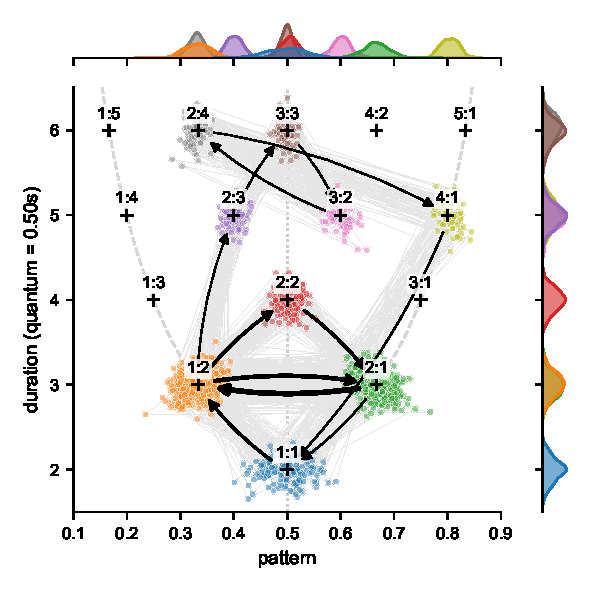
\includegraphics{../../figures/cluster-analysis.pdf}%
  }\\
  \caption{%
    \textbf{A cluster transition network.} 
    Noisy repetitions of a fixed rhythm are shown as a pattern-duration plot (cf. Figure~\ref{fig:plots}C-3). 
    This dataset is quantal and so durations (vertical axis) have been expressed as multiples of the quantum ($0.5$s). 
    All possible segments are marked and annotated: $2 : 3$, for example, indicates the segment $(1.0, 1.5)$ consisting of two and three quanta. 
    The marginal density plots show a ratio plot (top, cf. Figure~\ref{fig:plots}D-3) and the distribution of segment durations (right). 
    Colors indicate clusters, and a cluster transition network shows transitions between clusters, with the thicker lines indicating more frequent transitions. 
    Gray lines in the background show individual segment transitions.%
  }
  \label{fig:cluster-transition-network}
  \end{center}
\end{figure}

\subsection{Cluster transition networks}
%———————————————————————————————————————
One drawback of scatter plots is that you lose the sequential order of segments. 
\citet{Ravignani2017MusicPercept} show sequential order in his phase plots by connecting successive segments with lines. 
These trajectories can, however, quickly clutter a plot, and so I propose instead to summarize segment transitions in a \emph{cluster transition network}. 
The idea is to group segments into clusters and visualize cluster transitions as a weighted network. 
Figure~\ref{fig:cluster-transition-network} illustrates this for the repeated rhythm (cf. Figure~\ref{fig:plots}-3), with a Ravignani-style phase plot as light gray lines in the background. 

To create the network in Figure~\ref{fig:cluster-transition-network} segment clusters were identified using the clustering algorithm HDBSCAN \citep{McInnes20172017ICDMW,Pedregosa2011JMachLearnRes}.
Clusters are then used as nodes in a network, and edges are added between two clusters whenever segments from the two clusters succeed one another in the dataset. 
Edges are weighted by transition frequency and infrequent ones ($<15$) are pruned. 
Since this is a quantal dataset, the duration has been rescaled to show multiples of the quantum $q = 0.5$s. 
This allows us to annotate all integer ratio segments (e.g. $2 : 4$ indicates the segment $(2q, 4q)$) and highlights that clusters correspond to small integer ratio patterns—as is to be expected of a quantal dataset. 

At the top of Figure~\ref{fig:cluster-transition-network} we see a deterministic section of the rhythm, starting from around $2 : 3$. 
By reading only the second number in the annotated ratios, one can work out that the deterministic section follows a rhythm of the form $3:3:2:4:1$. 
The lower part of the network is more ambiguous and suggests multiple routes through the clusters around $1 : 1$, $1 : 2$, $2 : 2$, and $2 : 1$. 
In reality, however, the rhythm always takes the same path: it consists of two repetitions of the backbone of Steve Reich’s \emph{Clapping Music} followed by a $3:3:2:4$ section. 
Repeating the analysis with segments of length 3 further disambiguates the clusters at the bottom of the figure, but at the cost of additional clusters. 
This can be seen in Figure~\ref{fig:3d-pat-dur}, which shows a pattern-duration plot for length-3 segments \citep{Hunter2007ComputSciEng,Ikeda2024}.


\begin{figure}
  \begin{center}
  \resizebox*{9cm}{!}{%
    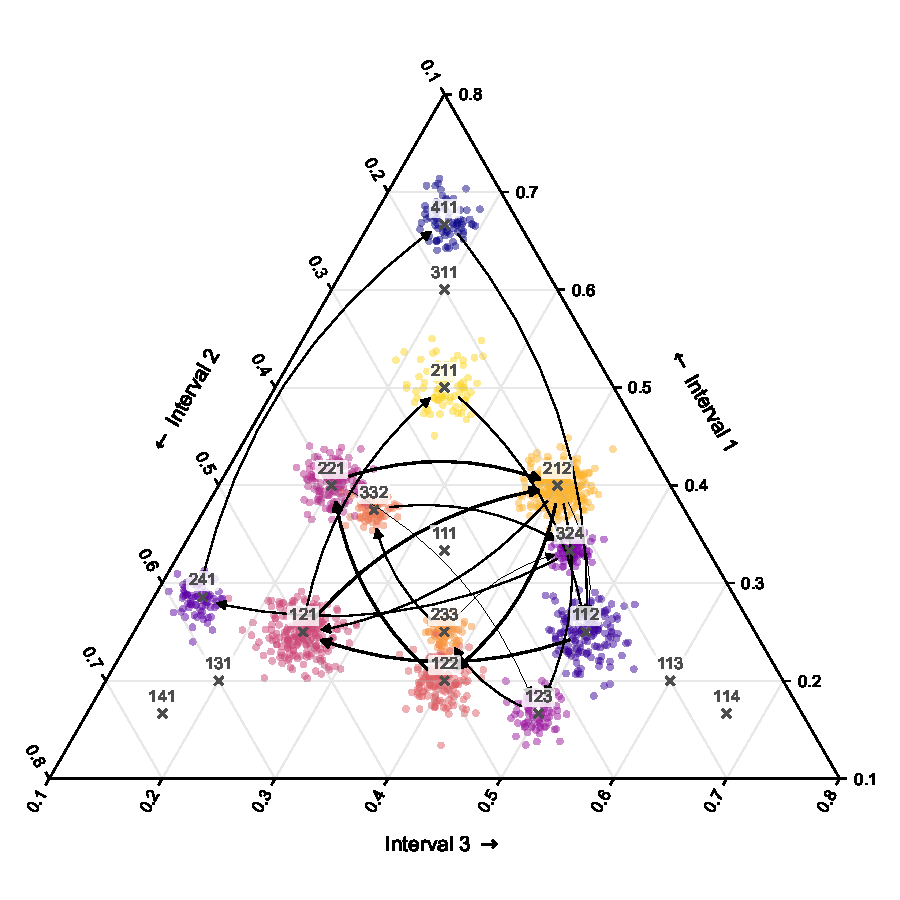
\includegraphics{../../figures/cluster-analysis-3d.pdf}%
  }\\
  \caption{%
    \textbf{A length-3 pattern-duration plot} of the repeated synthetic dataset. 
    The place in the rhythm triangle represents the pattern (the axes have been rotated with respect to Figure~\ref{fig:rhythm-triangle}) and color encodes the segment duration, expressed in multiples of the quantum. 
    Compared to Figure~\ref{fig:cluster-transition-network}, the additional time step further disambiguates the fastest clusters.%
  }
  \label{fig:3d-pat-dur}
  \end{center}
\end{figure}


\subsection{Case study: Cuban salsa and son}
%———————————————————————————————————————————
So far, I have only presented synthetic rhythmic data. 
To illustrate a more realistic use case of the pattern-duration plots, I turn to the IEMP Cuban salsa and son dataset \citep{Clayton2021EMR,Poole2019}.
The corpus consists of five songs in the styles of son and salsa, performed by the Cuban band Asere and contains automatically extracted onset annotations for all instruments separately. 
A length-2 pattern-duration plot was made using those onsets. 
I computed the 16th-note duration (the quantum) from the metrical cycle annotations, which allowed me to annotate integer ratio segments as before. 
HDBSCAN is used to cluster segments, with a minimum of 10 segments per cluster. 
This clustering method can decide not to assign a segment to a cluster. 
Such segments are marked with gray plus signs and ignored when computing the network.

Figure~\ref{fig:iemp-css} shows pattern-duration plots for four selected instruments across four songs (see \suppl{3} for more instruments).
For the cajon in the first song (Figure~\ref{fig:iemp-css}A), we see two cycles representing the rhythms $1:3:4$ and $1:3:2:2$, but we cannot see how they alternate. 
Note that the second rhythm is a variant of the first (it splits the final interval in half), and observe how this transforms the path through pattern-duration space. 
The clave in song 2 (Figure~\ref{fig:iemp-css}B) performs a consistent $3:3:4:2:4$ rhythm: precisely the 3-2 son clave pattern of this song \citep{Poole2019}. 
The tres (Figure~\ref{fig:iemp-css}C) and guitar (Figure~\ref{fig:iemp-css}D) play much faster rhythms of one or two 16th notes. 
Disambiguating the precise rhythms played would again require additional analyses, for example, using longer segments.


\begin{figure}
  \begin{center}
  \resizebox*{12cm}{!}{%
    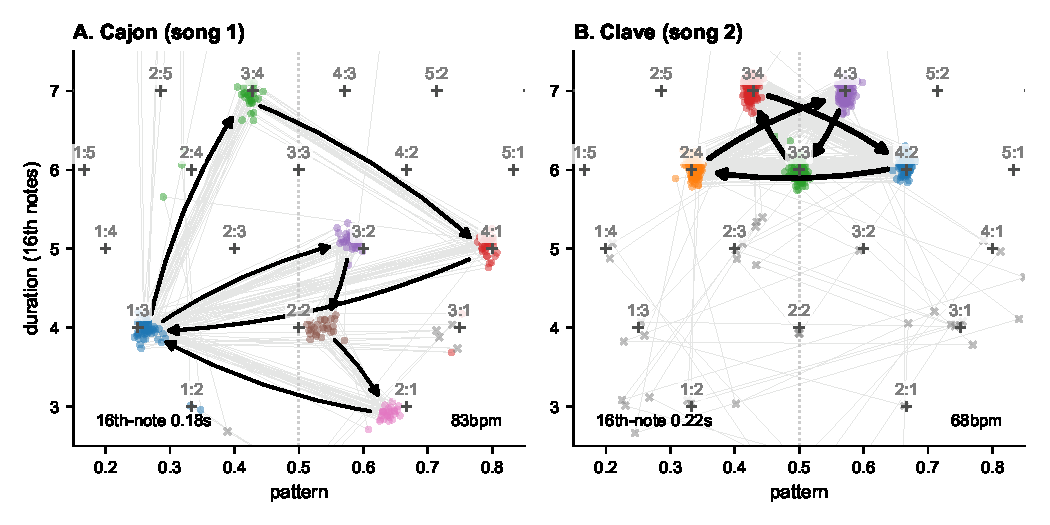
\includegraphics{../../figures/iemp-css/iemp-css-selection.pdf}%
  }\\
  \caption{%
    \textbf{Selected instruments} from the IEMP Cuban salsa and son corpus. 
    Pattern-duration plots for four instruments playing either relatively slow rhythms (cajon and clave, top) or relatively fast rhythms (bottom). 
    Expressing duration (vertically) in terms of the quantum (a 16th note) makes the plots directly comparable. 
    Clusters were identified automatically as discussed in the main text. 
    Note that one can follow the rhythm along a trajectory by ignoring the first number of every ratio. 
    Starting at $4 : 3$, the clave in panel \textbf{(B)} has the form $3:3:4:2:4$.
    }
  \label{fig:iemp-css}
  \end{center}
\end{figure}


%====================
\section{Measurement}%
\label{sec:measurement}
%====================


The visualization methods introduced in the previous section are probably best paired with quantitative measures. 
In this section I demonstrate how the distance measures on the simplex give rise to useful measures of rhythmic structure. 
A more detailed and formal exposition can be found in the Online Supplement.


\subsection{Anisochrony}
%———————————————————————
The most obvious quantity to measure is ‘regularity’: how isochronous is a given dataset? In terms of segments, one could measure the average distance of a set of patterns to the isochronous pattern at the center of the simplex. 
More precisely, that would measure anisochrony, how non-isochronous a pattern is. 
Formally, the \emph{anisochrony} of a pattern $(r_1, \dots, r_n)$ is the normalized distance from isochrony,
\[
\alpha(r_1, \dots, r_n) 
  = \frac{n}{2(n-1)} \sum_{i=1}^n \left|r_i - \tfrac{1}{n}\right|.
\]
Unpacking this, the absolute differences $|r_i - \frac{1}{n}|$ compare the pattern of interest to the isochronous pattern $(\tfrac{1}{n}, \tfrac{1}{n}, \dots, \tfrac{1}{n})$. 
The normalizing constant $n / (n - 1)$ ensures that the measure scales from $0$ in the center (perfectly isochronous) to $1$ (maximally anisochronous) in the corners of the simplex. 
Using the pattern distance explains the remaining factor of $\tfrac{1}{2}$. 

For interval pairs, the above definition can be dramatically simplified. 
The anisochrony of a pattern $(r, s)$ is simply the absolute difference between the relative durations:
\[
  \alpha(r, s) = |r-s|.
\]
For example, a rhythm ratio of $r = 0.5$ has anisochrony $0$ as it is perfectly isochronous. 
A ratio of $0.25$ has anisochrony $0.5$ and as the ratio approaches $0$, the anisochrony grows towards $1$.


\subsection{Reconstructing the nPVI}
%———————————————————————————————————
The proposed measure of anisochrony turns out to completely ‘reconstruct’ the normalized pairwise variability index \citep{Low2000LangSpeech}. 

Originally introduced to quantify speech rhythm, it became one of the standard measures of rhythmic regularity, in particular in music-language comparisons \citep[see e.g.][]{Condit-Schultz2019MusicPercept,VanHandel2022}.
For a sequence of intervals $i_1, \dots, i_K$, the nPVI is defined as 
\[
\text{nPVI} 
  = \frac{200}{K-1}  
    \sum_{k=1}^K \left| \frac{i_k - i_{k+1}}{i_k + i_{k+1}} \right|.
\]
We can see that the nPVI is $200$ times the average of some quantity: the expression inside the summation. 
That quantity is the absolute difference between the relative durations $i_k / (i_k + i_{k+1})$ and $i_{k+1} / (i_k + i_{k+1})$ of two intervals in a segment. 
As we showed above, this is exactly the anisochrony of a length-2 pattern. 
This means that the nPVI is $200$ times the average anisochrony, and so the nPVI \emph{measures average distance from isochrony}. 
This result moreover justifies replacing the nPVI with the anisochrony, as it more conveniently scales from $0$ to $1$. 
Alternatively, one could flip the definition to define the isochrony as one minus the anisochrony.

I first reported this result in \emph{{\color{red} my doctoral dissertation (2024; anonymized)}}
% Cornelissen (2024, ch. 8), %TODO REMOVE REF anonymous
but \citet{Jadoul2025Vibration} recently reached a closely related conclusion. 
They describe the nPVI as a summary statistic of rhythm ratios. 
To show that, it suffices to express the anisochrony of a pattern $(r, s)$ solely in terms of $r$. 
That is indeed possible: it is $2|r - 0.5|$. 
But what quantity does this represent? 
\citet{Jadoul2025Vibration} come very close to answering that question when they write that the nPVI quantifies how much the rhythm ratios “diverge from 0.5 (i.e. isochrony)” on average. 
It is a small step to observe that this “divergence” is a distance, but arguably an important one: it provides a geometric interpretation that is generalizable.


\subsection{Beyond the nPVI}
%————————————————————————————
Generality is one of the main benefits of the anisochrony measure introduced above: it is defined for arbitrarily long segments. 
The nPVI only quantifies ‘first order’ isochrony: when two successive intervals have the same length. 
Figure~\ref{fig:cluster-transition-network}
is an example of a dataset with substantial length-2 isochrony, as can be seen from the ratio plot at the top. 
Still, segments of \emph{three} identical intervals are completely absent, as can be seen in Figure~\ref{fig:3d-pat-dur}.
This is a distinction length-3 anisochrony can make, while the nPVI cannot. 
Put differently, the anisochrony gives a stricter assessment of isochrony than the nPVI when longer segment lengths are used.

The measure can be extended in a second direction: by changing the ‘reference’ pattern. 
Anisochrony measures the average normalized distance to one particular reference pattern, namely the isochronous one. 
Depending on the research question, other references may be more relevant. 
For example, perhaps the average distance to the $7 : 2 : 3$ \emph{maraka} rhythm could be an informative measure when studying music from Mali \citep[cf.][]{Jacoby2024NatHumBehav}.
Such measures will remain crude summaries and should probably be complemented by at least a visualization of the pattern distribution. 
A similar point is made by \citet{Jadoul2025Vibration}, who go on to suggest altogether different measures, such as the entropy of the pattern distribution—a suggestion left for future work. 


%===================
\section{Discussion}
%===================


In this paper, I proposed analyzing rhythmic data by studying its segments. 
This simple conceptual framework turned out to be remarkably productive. 
Decomposing segments into patterns and durations maps them to a convenient mathematical space, the rhythm simplex, that lends itself well to visualization. 
In particular, I introduced pattern-duration plots that effectively summarized regularities in instrument onsets, especially when overlaid with a cluster transition network. 
Finally, a number of quantitative measures are naturally explained by this framework. 
Rhythm ratios are simply length-2 patterns, and the nPVI is an average distance from isochrony, perhaps better replaced with the more general and normalized anisochrony measure. 

Still, the main contribution is neither the plotting method nor the measures, but the simple concepts of segments and patterns: they tie together the work on which this paper builds and they may simplify our reasoning about rhythmic data. 
This paper can also be read as an argument for visualizing rhythmic data before using quantitative measures such as the nPVI. 
Moreover, it underlines that the nPVI or its proposed replacement, the anisochrony, should only be used when you actually need to assess isochrony. 
Otherwise, this paper provides the conceptual tools for developing more appropriate measures. 
Future work could explore extending the framework, for example by combining segments of different lengths, or studying segments that skip one or more intervals (i.e. skip-grams). 

% \subsection{Criticism of the nPVI}

Since the anisochrony effectively generalizes the nPVI, the criticism of the nPVI raised by \citet{Condit-Schultz2019MusicPercept} may carry over to the present paper. 
However, a central part of the critique concerns the application of an average to discrete intervals in notated rhythm. 
For the continuous data analyzed here, this seems less problematic. 
More generally, \citet{Condit-Schultz2019MusicPercept} argues for using standard measures like the nPVI critically, advocates a plurality of measures, and stresses the importance of musically relevant rhythmic features over general measures. 
All of this, in fact, aligns well with the kind of rhythmic segment analyses I argue for here.

% \subsection{Cognitive plausibility}

Throughout this paper, I have tried to avoid making cognitive claims. 
One reason for this is domain generality: the aim was a framework that made as few assumptions as possible, so that it would be applicable to any kind of rhythmic data. 
In particular, I do not claim that the pattern distance is a good model of perceived dissimilarity. 
To the extent that rhythm is perceived categorically, it clearly is not: perceived dissimilarity might then be increased across category boundaries \citep{Desain2003Perception},
while the pattern distance remains unaffected by such boundaries. 
This may actually be desirable: to operationalize a notion such as increased dissimilarity across a category boundary requires a neutral distance measure. 
If anything, it is clear how perceptual models could enter the framework. 
Finally, an aspect that may lend itself more directly to cognitive interpretation is the distinction between patterns and durations (tempo).

% \subsection{Quantal data and small integer ratios}

This paper also introduced the concept of quantality to describe rhythmic data that approximately falls on a regular grid. 
Throughout the paper, the quantum was taken to be constant, which implies a constant tempo. 
This is an unrealistic assumption for a lot of music, and so future work could consider expressing segment durations in terms of a time-varying quantum. 
After all, the concept itself seems productive. 
Pattern-duration plots, for example, are more insightful when all integer-ratio segments are annotated, which requires a quantum. 
Indeed, quantality turns out to be very closely connected to the presence of small integer ratio rhythms—a topic of much recent \emph{perceptual} research \citep{Jacoby2024NatHumBehav,Jacoby2017CurrBiol,Ravignani2018FrontComputNeurosci}.
The two notions appear to be two sides of the same coin. 
This suggests that questions about integer ratios can be reformulated as questions about quantality, and it connects the present work to fundamental questions about music.


%%%%%%%%%%%%%%%%%%%%%%%%%%%%%%%%%%%%%%%%%%%%%%%%%%%%%%%%%%%%%%%%%%%%%%%%%%%%%%%%%%%%%
%%%%%%%%%%%%%%%%%%%%%%%%%%%%%%%%%%%%%%%%%%%%%%%%%%%%%%%%%%%%%%%%%%%%%%%%%%%%%%%%%%%%%


\section*{Acknowledgements}
\addcontentsline{toc}{section}{Acknowledgements}
%———————————————————————————————————————————————

\anonymized{}
% I would like to thank Henkjan Honing for his support of this work and for valuable feedback on the terminology and presentation.
%.I thank [names] for constructive comments on previous versions of this paper.
%I would like to thank the two anonymous reviewers and Editor [name] for \dots



\section*{Funding}
\addcontentsline{toc}{section}{Funding}
%——————————————————————————————————————

\anonymized{}

% TODO 
% Bas Cornelissen was supported by the Dutch Research Council (NWO) through an Open Competition grant (406.20.CW.002) awarded to Henkjan Honing. 


\section*{Supplemental online material}
\addcontentsline{toc}{section}{Supplemental online material}
%———————————————————————————————————————————————————————————

Supplemental online material for this article can be accessed at \url{doi-provided-by-publisher}.
The Online Supplement provides a more formal exposition of the ideas in this paper, as well as additional figures and analysis supporting the findings reported in this paper.
All data and code used in this paper have been deposited at \url{doi.org/10.5281/zenodo.anonimized}.
% doi.org/10.5281/zenodo.17753529. 

% TODO is my phrasing correct?
% Use this exact phrasing.
% The official Online Supplement file will be hosted at the article link provided by the publisher. You may also host other material at your-own-link.

\section*{Disclosure statement}
\addcontentsline{toc}{section}{Disclosure statement}
%———————————————————————————————————————————————————

No potential conflict of interest was reported by the authors. 

{\bigbreak\noindent\color{red}%
  \textbf{@EDITOR: I would like to be transparent about the use of AI tools. 
Where would a statement like this fit best?}

  OpenAI’s Codex model assisted the development some of the research code, but always instructed and supervised by the author: part of the Python package was for example written in collaboration with Codex, in particular the documentation and test suites. 
ChatGPT was used when brainstorming terminology and presentation of the ideas in this paper: the term ‘quantal’ was for example suggested by ChatGPT. 
The paper was, however, entirely written by the author, without assistance from a chatbot except for the very final spelling and grammar check.
}

\section*{ORCID}
\addcontentsline{toc}{section}{ORCID}
%————————————————————————————————————

Do not change this. Production will take care of it if the paper is accepted.

% References
%————————————————————————————————————
\bibliographystyle{tMAM}
\bibliography{references}
\addcontentsline{toc}{section}{References}

\end{document}
